\chapter{Methodik}\label{ch:method}

\section{Theoretischer Hintergrund}

Zur Auswertung der Daten werden drei verschiedene Machine-Learning-Algorithmen entweder einzeln oder in Kombination verwendet: die lineare Regression, das CNN und das LSTM.

\subsection{Logistische Regression}

Im Gegensatz zur bekannteren linearen Regression bietet sich die logistische Regression deutlich mehr für die Zwecke dieser Arbeit an.
Die lineare Regression ist darauf ausgelegt, quantitative Werte wie Verkaufszahlen vorauszusagen. Dazu sagt sie auch Werte außerhalb des Bereichs von 0 bis 1 voraus. Bei Straßenbelägen handelt es sich aber um qualitative Variablen. Diese stehen in keinem quantitativen Zusammenhang und sind unabhängig voneinander. Um mit diesen "Werten" arbeiten zu können, braucht man eine Methode, die nicht die Werte direkt, sondern Wahrscheinlichkeiten voraussagt, mit denen eine Beobachtung zu einem der Werte gehört.

\begin{figure}[htbp]
    \centering
    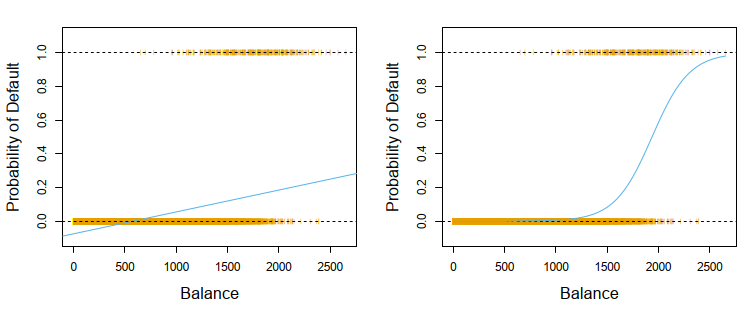
\includegraphics[width=0.8\textwidth]{figures/Linear_vs_logistic.png}
    \caption{Vergleich der geschätzten Wahrscheinlichkeiten für einen Testdatensatz zwischen linearer Regression (links) und logistischer Regression (rechts). \cite{James2023}}
    \label{fig:Vergleich_lin_log}
\end{figure}

Wie in \ref{fig:Vergleich_lin_log} zu sehen, können bei der linearen Regression die vorausgesagten Wahrscheinlichkeiten sogar negativ werden. Auch wird der gesamte Bereich von 0 bis 1 nicht ausgenutzt. Die logistische Regression löst dieses Problem. Um die benötigten Werte zwischen 0 und 1 vorherzusagen, setzt die logistische Regression die "logistische Funktion" ein:

\begin{equation}
    p(X) = \frac{e^{\beta_0 + \beta_1 X}}{1 + e^{\beta_0 + \beta_1 X}}
    \label{eq:logistische_funktion}
\end{equation}

Wie in Gleichung (\ref{eq:logistische_funktion}) zu sehen ist, nähert sich die Funktion für sehr große Werte von $X$ der 1 an und für sehr kleine Werte der 0. Durch Umformung lässt sich die logistische Funktion als lineares Modell formulieren. Der Ausdruck auf der linken Seite wird als Log-Odds bezeichnet:

\begin{equation}
    \log\left(\frac{p(X)}{1 - p(X)}\right) = \beta_0 + \beta_1 X
    \label{eq:log_odds}
\end{equation}

Wie in Gleichung (\ref{eq:log_odds}) ersichtlich ist, stellt das logistische Regressionsmodell sicher, dass der Logit linear von den Eingabevariablen $X$ abhängt.
Hierbei sind $\beta_0$ und $\beta_1$ die Koeffizienten oder Gewichte, die mit den Trainingsdaten bestimmt werden müssen. Das $X$ ist der Eingabewert (oder das Feature), dessen Zugehörigkeit bestimmt werden soll. Damit dies korrekt geschieht, wird die Maximum-Likelihood-Methode angewendet.

\begin{equation}
    l(\beta_0, \beta_1) = \prod_{i: y_i=1} p(x_i) \prod_{i': y_{i'}=0} (1 - p(x_{i'}))
    \label{eq:likelihood}
\end{equation}

Hierbei repräsentiert $p(x_i)$ die vorhergesagte Wahrscheinlichkeit für eine Beobachtung $i$, deren tatsächliche Klasse $y_i = 1$ ist, und $(1 - p(x_{i'}))$ die Wahrscheinlichkeit für eine Beobachtung $i'$, deren tatsächliche Klasse $y_{i'} = 0$ ist. Hat man die Koeffizienten erfolgreich bestimmt, muss man zum Klassifizieren nur noch den zu bestimmenden Wert in die X-Variable der logistischen Funktion einsetzen, um die Wahrscheinlichkeit zu erhalten, ob der Wert zu einer bestimmten Klasse gehört oder nicht.

Da in dieser Arbeit mit mehr als zwei Klassen gearbeitet wird, kommt die sogenannte multinomiale logistische Regression zum Einsatz. Es gibt hier verschiedene Ansätze, doch es läuft auf dasselbe Prinzip hinaus: Den einzelnen Klassen werden in ihrem Zusammenhang noch einmal einzelne Wahrscheinlichkeiten für ihren Eintritt zugewiesen. Dies geschieht entweder durch eine zufällig ausgewählte Klasse K als Basisklasse, mit der verglichen wird, oder komplett symmetrisch ohne eine einheitliche Referenz (die sogenannte Softmax-Methode).

Für die Methode mit $K$ Klassen und einer Klasse als Referenzklasse (hier Klasse $K$) berechnet man die Log-Odds für jede der verbleibenden $K-1$ Klassen im Verhältnis zu dieser Referenzklasse:

\begin{equation}
    \log\left(\frac{\Pr(Y=k|X=x)}{\Pr(Y=K|X=x)}\right) = \beta_{k0} + \beta_{k1}x_1 + \dots + \beta_{kp}x_p
    \label{eq:multinomial}
\end{equation}

Dabei beschreiben die Parameter $\beta_{k0}, \dots, \beta_{kp}$ die Koeffizienten spezifisch für die Klasse $k$.
Bei Softmax wird die Wahrscheinlichkeit für jede Klasse $k$ direkt berechnet, ohne eine Referenzklasse zu definieren:

\begin{equation}
    \Pr(Y=k|X=x) = \frac{e^{\beta_{k0} + \beta_{k1}x_1 + \dots + \beta_{kp}x_p}}{\sum_{l=1}^{K} e^{\beta_{l0} + \beta_{l1}x_1 + \dots + \beta_{lp}x_p}}
    \label{eq:softmax}
\end{equation}

Die Funktion in Gleichung (\ref{eq:softmax}) stellt sicher, dass die berechneten Wahrscheinlichkeiten für alle $K$ Klassen exakt auf 1 summieren. \footnote{\cite{James2023}}

Da es sich bei der logistischen Regression um eine vergleichsweise simple und transparente mathematische Funktion handelt, ist sie sehr leichtgewichtig. Sie arbeitet schnell, verbraucht nicht viel Speicher und lässt sich leicht in viele verschiedene Endgeräte integrieren. Daher wird sie in dieser Arbeit als erste Möglichkeit eingesetzt.

\subsection{Convolutional Neural Network}
Das Neural Network ist das Standardwerkzeug im Bereich des Deep Learning.

\begin{figure}[htbp]
    \centering
    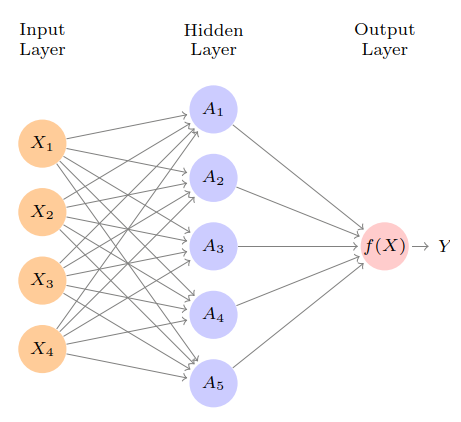
\includegraphics[width=0.6\textwidth]{figures/Neural_Network.png}
    \caption{Neural Network mit einem Hidden Layer. \cite{James2023}}
    \label{fig:neural_network}
\end{figure}

In seinen Grundsätzen besteht es aus einem Input Layer, einem oder mehreren Hidden Layern und einem Output Layer. Wie in Abbildung \ref{fig:neural_network} zu sehen ist, nimmt das Network eine Anzahl $p$ an Inputs $X = (X_1, \dots, X_p)$ und bildet im Hidden Layer eine nicht-lineare Transformation für die Kombination dieser Inputs in jedem Knoten $A$. Die Ergebnisse dieser sogenannten Aktivierungen werden an das Output Layer weitergereicht, um die nicht-lineare Funktion $f(x)$ zu bilden. Diese kann die Antwort $Y$ voraussagen. Die Aktivierungsfunktionen in den $K$ Knoten $A_k, k=1, \dots, K$ werden im Vorhinein festgelegt. Heutzutage verwendet man am häufigsten die ReLU-Funktion (Rectified Linear Unit):

\begin{equation}
    g(z) = (z)_+ = \begin{cases} 
        0 & \text{falls } z < 0 \\ 
        z & \text{sonst}
    \end{cases}
    \label{eq:relu}
\end{equation}

Diese ist einfacher zu berechnen und auch platzsparender als die vorher genutzte Sigmoid-Funktion. Das Modell aus Abbildung \ref{fig:neural_network} beschreibt, wie aus den fünf Kombinationen von $X$ fünf neue Features berechnet werden. Diese werden dann mit einer Aktivierungsfunktion transformiert. Am Ende ergibt sich ein lineares Modell zum Berechnen der Wahrscheinlichkeiten, ob ein Input zu einer Klasse gehört oder nicht.\footnote{\cite{James2023}}

Die meisten neuronalen Netze haben jedoch eine Vielzahl an Hidden Layern, um komplexere Aufgaben zu lösen, und auch mehrere mögliche Outputs, um Daten einer Vielzahl an möglichen Klassen zuzuordnen. Hierzu wird wieder die Softmax-Funktion aus Gleichung (\ref{eq:softmax}) verwendet, um für jede mögliche Klasse die Wahrscheinlichkeit zu errechnen, um dann den Input zur Klasse mit der höchsten Wahrscheinlichkeit zuzuweisen.

\begin{figure}[htbp]
    \centering
    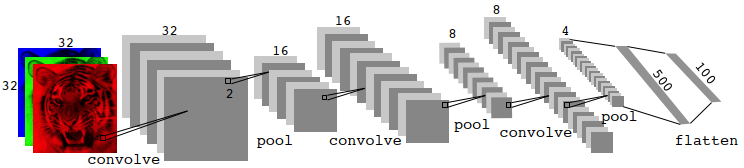
\includegraphics[width=0.8\textwidth]{figures/CNN.png}
    \caption{Struktur eines tiefen CNNs mit einer Abfolge von Convolutional Layers und Pooling Layers. \cite{James2023}}
    \label{fig:cnn}
\end{figure}

Das CNN zeichnet sich durch seine Eignung zur Klassifizierung mehrdimensionaler Daten aus. Anders als reguläre neuronale Netze werden die Hidden Layers hier in Convolutional Layers und Pooling Layers unterteilt. Diese Unterteilung ermöglicht ein hierarchisches Identifizieren von Features, von Low-Level nach High-Level, wobei mehrere Low-Level-Features zu High-Level-Features kombiniert werden, um schrittweise komplexere Muster zu erkennen. Die Convolutional Layers nutzen kleine Filtermatrizen (Kernels genannt), um schrittweise über die Daten zu gehen, die Werte, auf denen sie sich befinden, mit den Werten des Filters zu multiplizieren und die Produkte aufzusummieren. Je höher diese Summe, desto ähnlicher sind die originalen Daten dem Filter. Je niedriger, desto mehr unterscheiden sie sich. Während des Trainingsvorgangs passen sich die Filter an, um immer differenzierter lokale Muster zu erkennen und zu extrahieren. Als Ergebnis bekommt man eine Feature Map, die die gefundenen Muster aufzeigt.

Das Pooling Layer fasst eine Feature Map zu einem kleineren Bild zusammen. Mit dem Max-Pooling-Verfahren werden 2$\times$2-Blöcke an Daten erfasst und auf den höchsten vorhandenen Wert reduziert. So bleiben alle wichtigen Daten erhalten. Diese Schritte werden in mehreren aufeinanderfolgenden Layern wiederholt, bis die Feature Map auf ein Minimum reduziert wurde. Die Map wird dann von ihrer mehrdimensionalen Struktur in eine eindimensionale Reihe an Daten überführt und in ein neuronales Netz gespeist, ähnlich wie oben beschrieben. Am Ende erhält man wieder eine Reihe an Wahrscheinlichkeitsfunktionen für die möglichen Klassen.\footnote{\cite{James2023}}

Das CNN findet seine Anwendung meistens im Klassifizieren von Bildern und nicht in sequenziellen Datenreihen. Da beide aber in ihrer Struktur eine mehrdimensionale Abfolge an Daten darstellen, wird auch der Einsatz in diesem Fall untersucht.

\subsection{Long Short Term Memory}


\section{Aufbau des Experiments}
Die Messreihen werden mit einem Citybike der Marke Pegasus Solero SL 7 aufgenommen. Das Fahrrad hat eine Rahmengröße von 280 mm und eine Reifengröße von 28 Zoll. Es wiegt ca. 18 kg. Mit dem Gewicht des Fahrers kommt man aufsummiert auf ca. 100 kg. Ein Smartphone der Marke Samsung Galaxy S23 kommt als Aufnahmegerät zum Einsatz. Es ist mit einer LSM6DSO Inertial Measurement Unit (LMU) ausgestattet, das Messung von Beschleunigung (Accelerometer) und Neigung (Gyroskop) in je 3 Achsen ermöglicht. \footnote{\cite{STMicroelectronics2023}}

Zugriff auf die Sensoren des Smartphones inklusive einstellbarer Aufnahmen von Messreihen wird durch die App "PhyPhox" der Universität RWTH Aachen ermöglicht. Das LMU erlaubt Aufnahmen bis zu einer Frequenz von 6.66 kHz. Dies ist für die Zwecke dieser Arbeit entschieden zu hoch. Aufbauend auf der Arbeit von Tarkiainen wurde sich für eine Aufnahmefrequenz von 150 Hz entschieden, um neben größeren Störungen wie Schlaglöchern und Bordsteinkanten auch granuläre Bodeneigenschaften erkennen zu können. Phyphox ermöglicht die simultane Aufnahme mehrerer Sensorarten. Für das Experiment werden der Accelerometer, das Gyroskop und das GPS des Smarphones als Daten verwendet. Hierbei wird darauf geachtet, dass die Option für das Verwenden purer Satteliten-Daten zur Standort- und Geschwindigkeitsbestimmung verwendet wird, um nicht verfälschende Signale von weniger präzisen Quellen wie WLAN oder Mobilfunk zusätzlich aufzunehmen.

\begin{figure}[htbp]
    \centering
    % Linke Minipage
    \begin{minipage}[b]{0.45\textwidth}
        \centering
        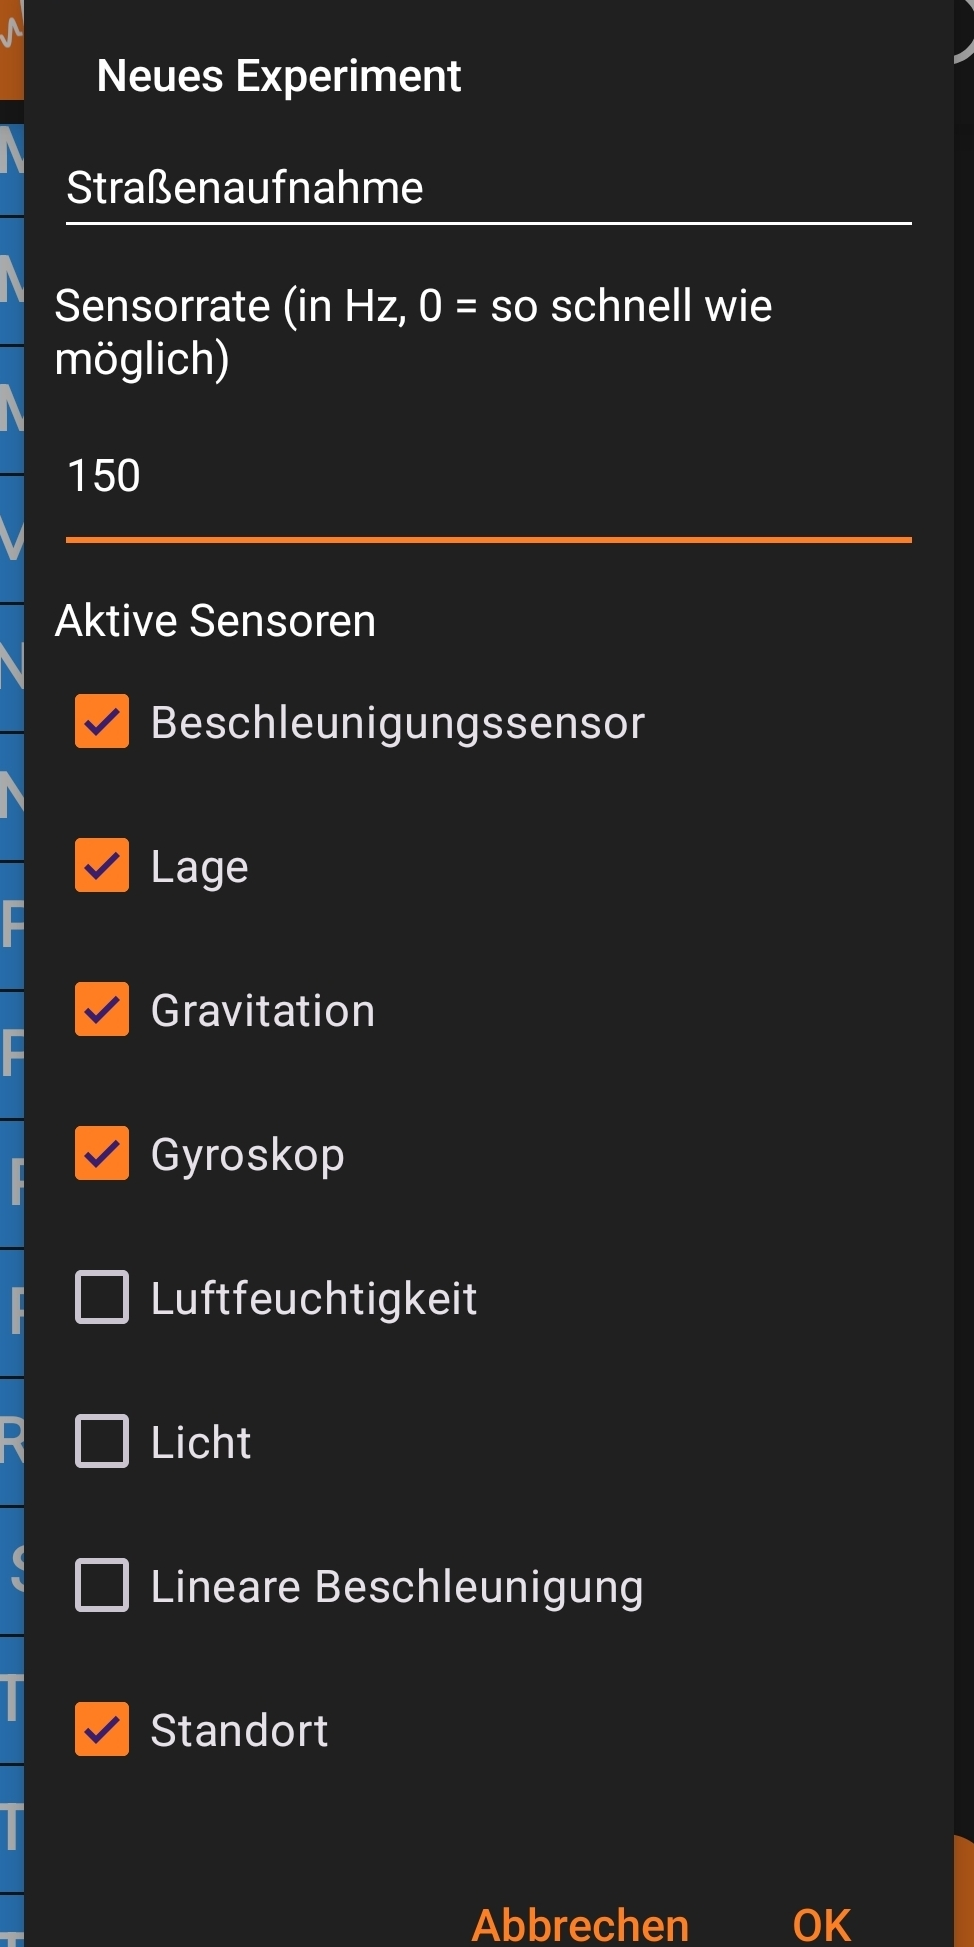
\includegraphics[width=0.7\textwidth]{figures/Screenshot_20260405_180917_phyphox.jpg}
        \caption{Einstellungen für die Messungen in PhyPhox.}
        \label{fig:setup}
    \end{minipage}
    \hfill
    \begin{minipage}[b]{0.45\textwidth}
        \centering
        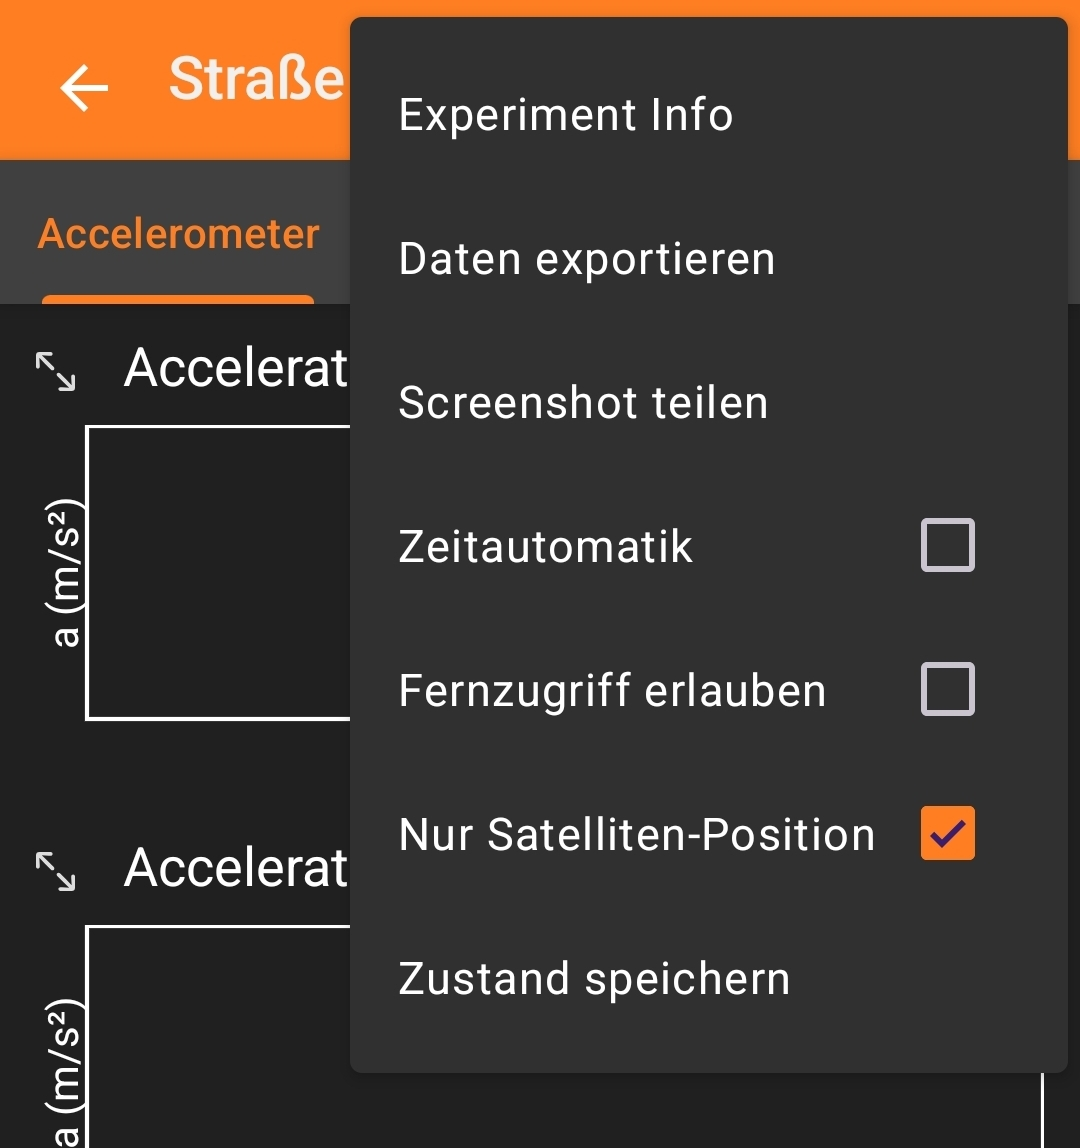
\includegraphics[width=0.7\textwidth]{figures/Screenshot_20260405_180641_phyphox.jpg}
        \caption{Option für die Aufnahme purer GPS-Daten.}
        \label{fig:setup2}
    \end{minipage}
\end{figure}

Zusätzlich wird der Schwerkraft-Sensor während der Fahrt aufgenommen, um einen Ankerpunkt für die Projektion der Accelerometer-Daten zu gewährleisten. 

Als Halterung für das Handy wird eine handelsübliche Lamicall-Halterung für Motorräder und Fahrräder verwendet. Das Smartphone wird in einem Winkel von ca. 45° angebracht, sodass das Smartphone vertikal in Fahrtrichtung zeigt.

\begin{figure}[htbp]
    \centering
    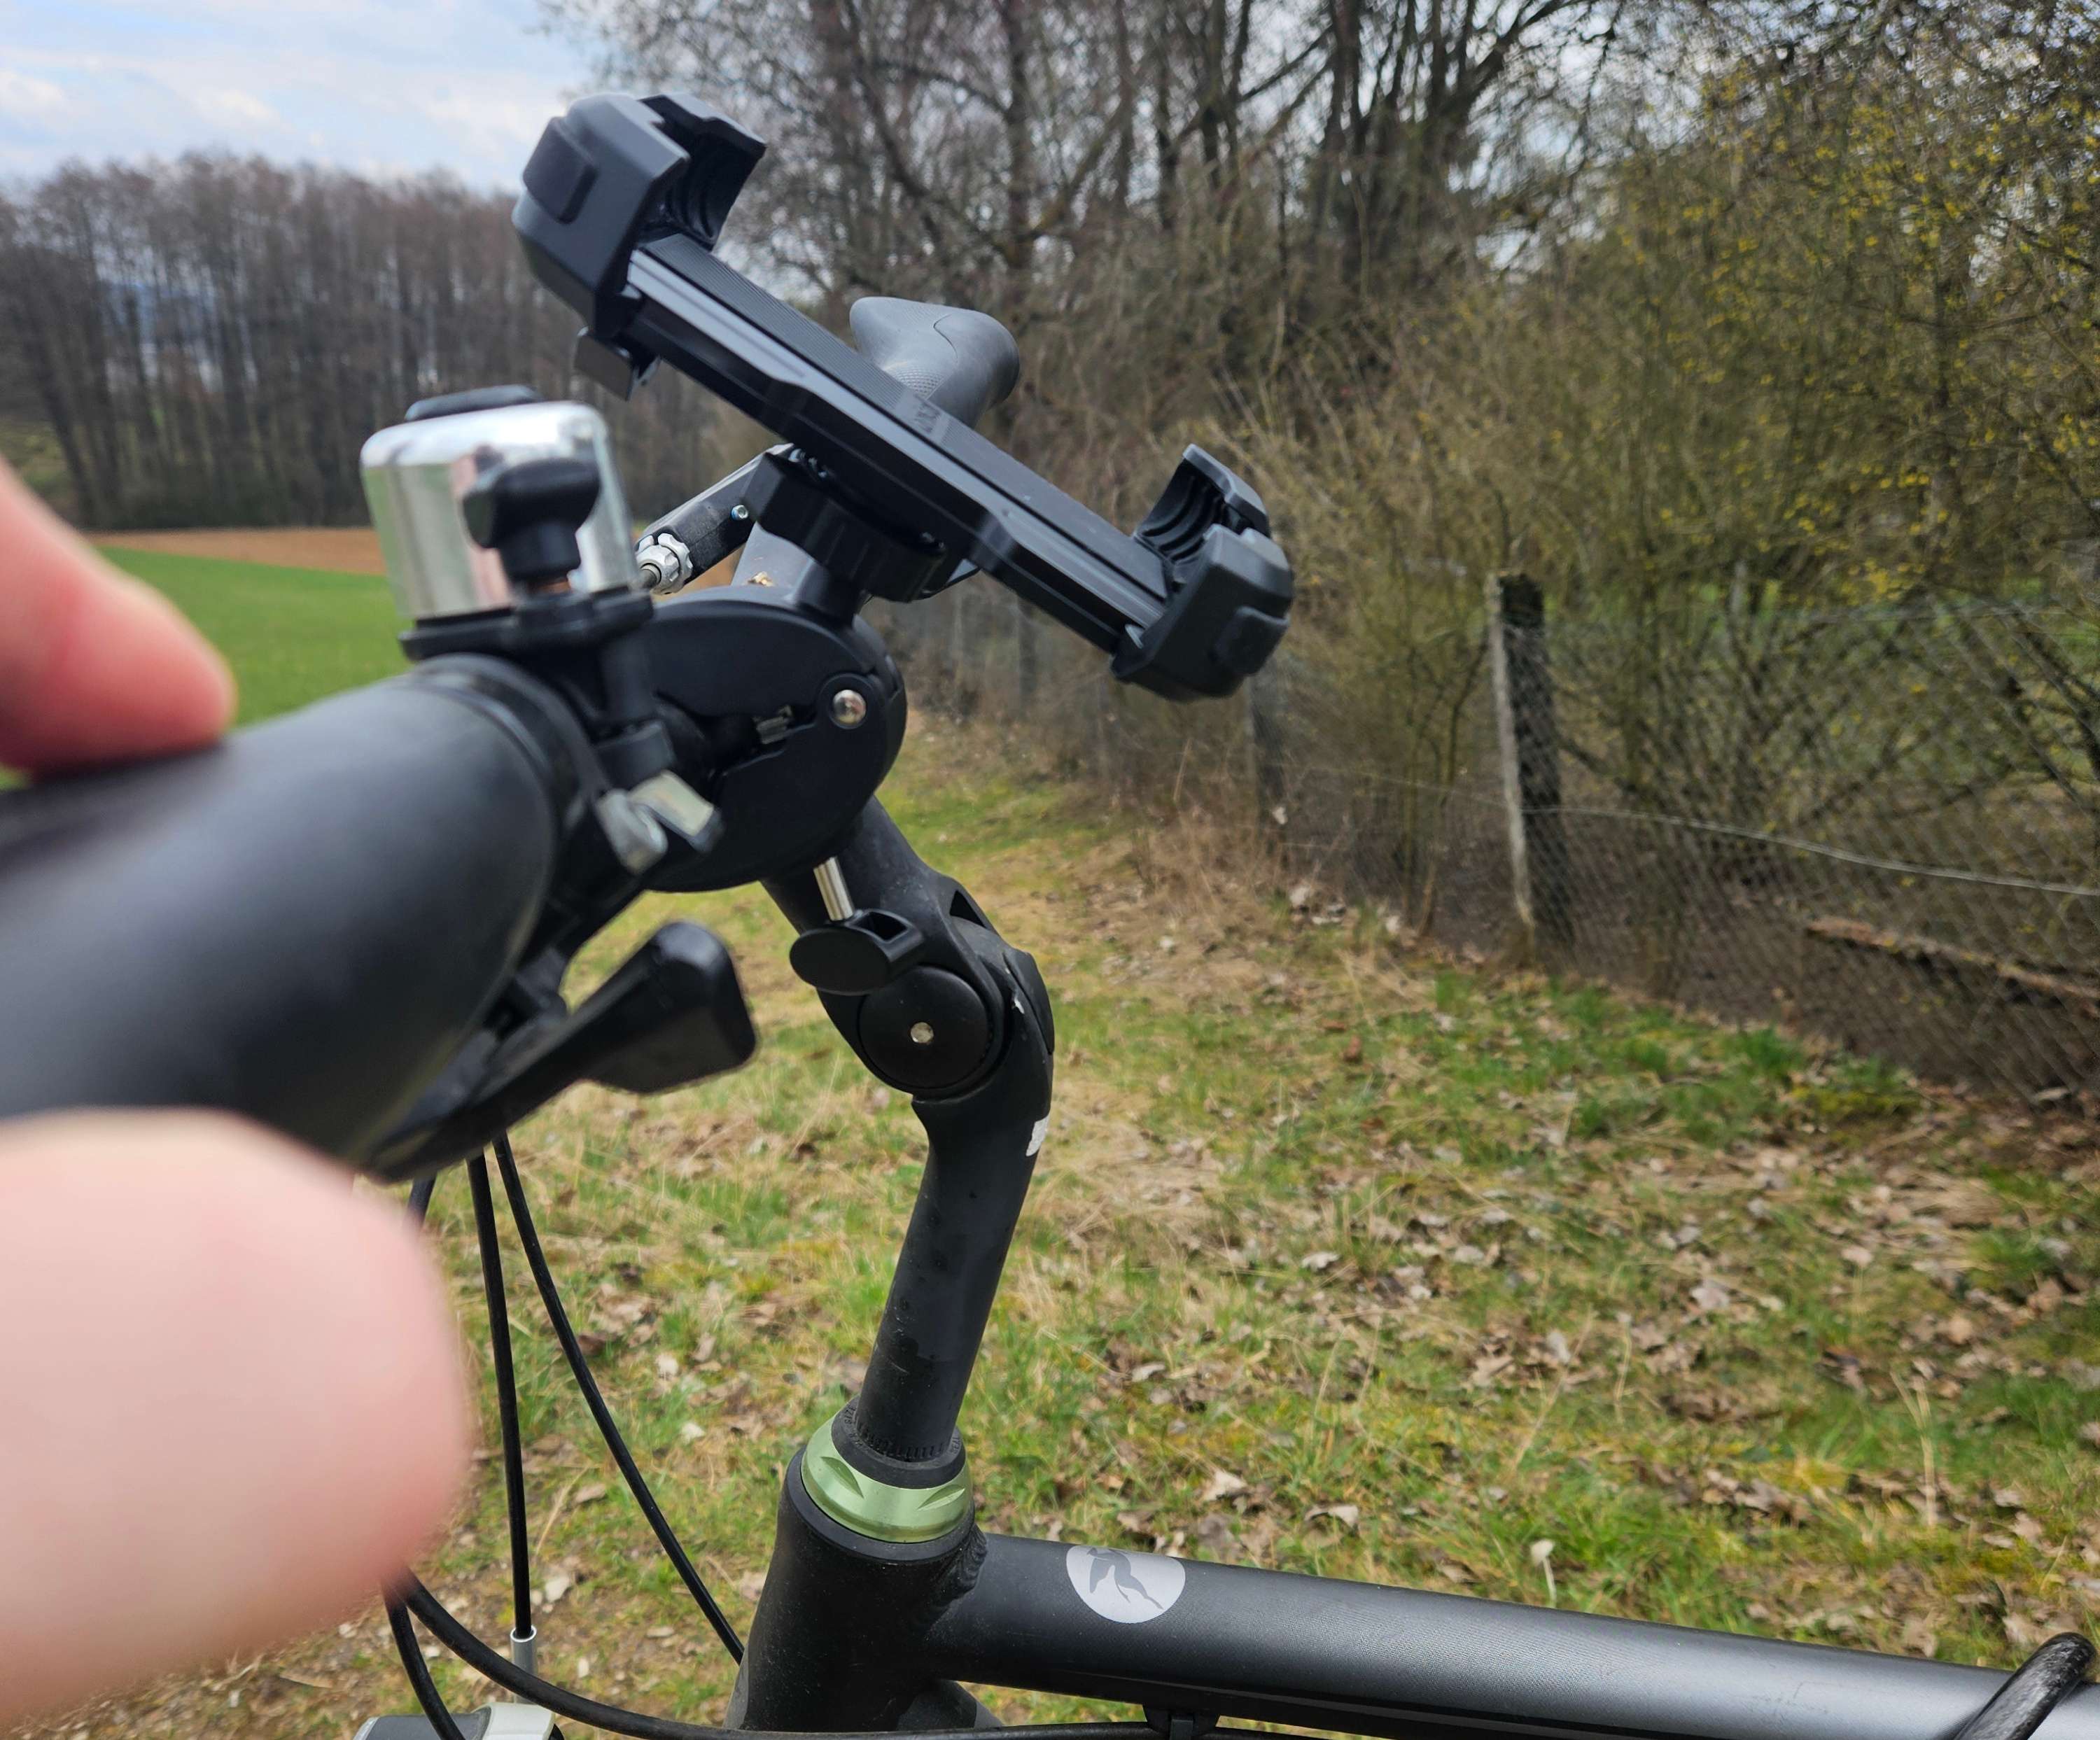
\includegraphics[width=0.4\textwidth]{figures/Halterung.jpg}
    \caption{Position der Halterung am Fahrrad.}
    \label{fig:halterung}
\end{figure}